\textbf{Drehbuch}
\begin{enumerate}
\item Fragen zum Buch.
\item Lernseqünz: Berechnung mittels Vektorisierung (geleitet).
\item übung 1: Wurfparabel (geleitet).
\item Kap. 6 (Funktionen und Fehlerhandling) vom Buch „Die nicht zu kurze Kurzeinführung in MATLAB“ selbstständig durcharbeiten.
\end{enumerate}
\textbf{Lernziele}
Die Studierenden...
\begin{enumerate}
\item festigen den Umgang mit Matlab.
\item erkennen, das viele Schleifen in Matlab nicht ausgeführt werden müssen.
\item verstehen die Mächtigkeit von Vektoroperationen.
\item und ebenso Darstellungsmöglichkeiten von ganzen Matrizen.
\item wissen, was ein m-File ist und können eine Funktion erstellen.
\end{enumerate}
\section{Wurfparabel}
Die Wurfparabel stellt den Verlauf eines Balles dar, der mit einer gewissen Anfangsgeschwindigkeit und einem gewissen Abschusswinkel geworfen wird.
Der Weg, den dieser Ball beschreibt, kann folgendermassen ausgedrückt werden:
\begin{equation}
sx\left(t\right)=\Big\vert\overrightarrow{v}\Big\vert\cdot \cos\left(\alpha\right)\cdot t
\end{equation}
\begin{equation}
sy\left(t\right)=\Big\vert\overrightarrow{v}\Big\vert\cdot\sin\left(\alpha\right)\cdot t-\dfrac{g}{2}\cdot t^2 
\end{equation}
$sx(t)$: $x$-Komponente der Wurfbahn [m].\\
$sy(t)$: $y$-Komponente der Wurfbahn [m].\\
$\Big\vert \overrightarrow{v}\Big\vert$ : Betrag der Wurfgeschwindigkeit [m/s].\\
$\alpha$: Abschusswinkel [grad, rad].\\
$t$: Zeit [s].\\
$g = 9.81$: Gravitationskonstante [m/s2
]\\\\
Programmieren Sie in MATLAB ein M-File, welches die Wurfparabel darstellt. Die Anzahl der
dargestellten Parabeln soll im M-File verändert werden können. Bei welchem Abschusswinkel
wird die Wurfweite maximal?  
\begin{center}
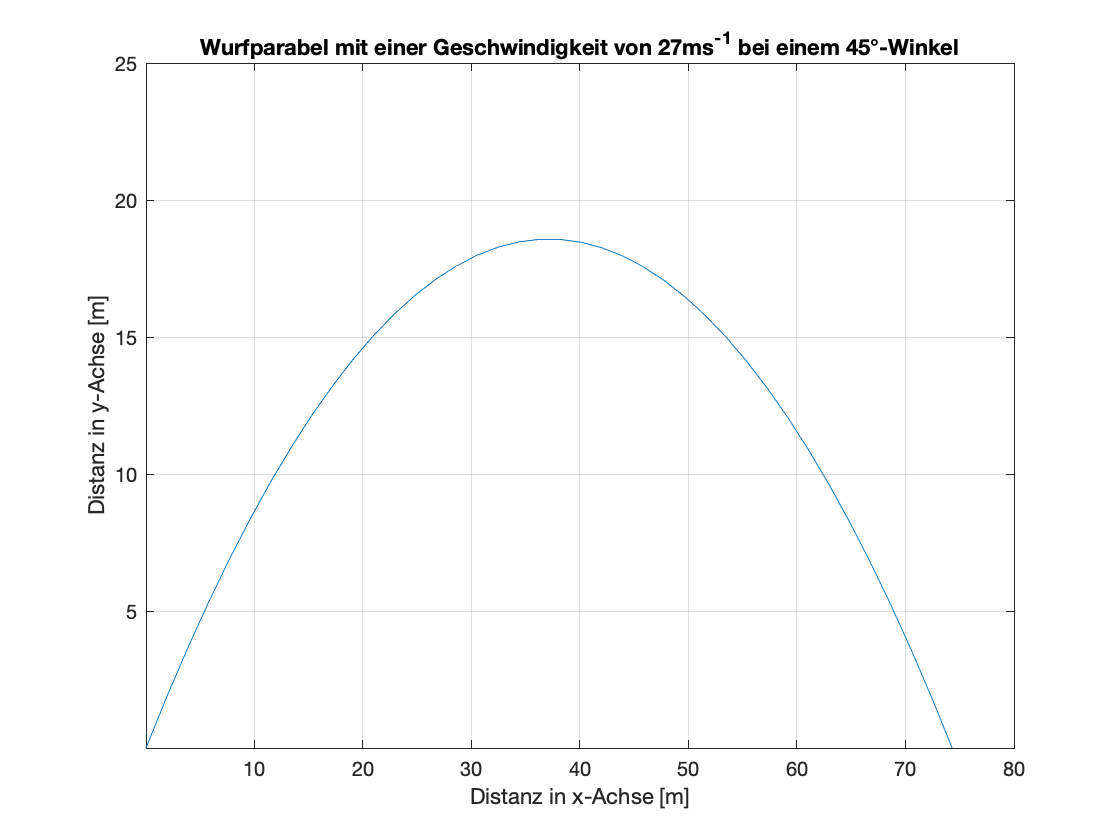
\includegraphics[scale=0.3]{../../PROJEKTE/ubungm3wurfparabel/ubungm3wurfparabel.png}
\end{center}
\lstinputlisting[language=Matlab, caption={Wurfparabel für 60 Grad}]{../../PROJEKTE/ubungm3wurfparabel/ubungm3wurfparabel.m}
\section{M3a) übung zu Funktionen}
öffnen Sie die Funktion {\color{magenta}\texttt{linspace}} mit dem Befehl {\color{magenta}\texttt{edit linspace}} und analysieren Sie diese Funktion von Mathworks. 
\lstinputlisting[language=Matlab, caption={übung M3a)}]{../../PROJEKTE/ubungm3a/ubungm3a.m}
Beantworten Sie folgende Fragen
\begin{enumerate}[$a)$]
\item Wie lang ist die Länge eines Standardvektors, wenn {\color{magenta}{keine Länge}} definiert wird?
\\
$\Longrightarrow$ Generierung eines Vektors mit 100 linear gleichabständigen Punkten.
\item Mit {\color{magenta}\texttt{help linspace}} erscheint die Hilfe dieser Funktion im Command Window 
\begin{enumerate}[$\bullet$]
\item Wo befindet sich dieser Text in der Datei?
\\
$\Longrightarrow$ Der angezeigte Text befindet sich im Command Window.
\item Ab welcher Zeile wird der Hilfetext nicht mehr ausgegeben? Wie wird dies abgegrenzt?
\\
$\Longrightarrow$ Eine Zeile vor der Zeile des Copyrights wird nichts mehr angezeigt. Durch {\color{magenta}\texttt{edit help}} kann man dies ändern.
\end{enumerate}
\end{enumerate}
\section{M3b) übung zu Kapitel 6}
Schreiben Sie eine Funktion welche die zwei Zahlen \texttt{a} und \texttt{b} addiert ({\color{magenta}\texttt{add}}), subtrahiert ({\color{magenta}\texttt{sub}}), multipliziert ({\color{magenta}\texttt{mult}}), dividiert ({\color{magenta}\texttt{div}}) und potenziert ({\color{magenta}\texttt{pow}}). Testen Sie diese Funktion gründlich. 
\lstinputlisting[language=Matlab, caption={übung M3a)}]{../../PROJEKTE/ubungm3b/ubungm3b.m}
\section{M3b) übung publish-pdf zu Kapitel 6}
Testen Sie Ihre Funktion nun selber, indem Sie die Testfunktion für die übung M3b) (oberhalb dieses Textblockes) herunterladen und mittels der Publish Funktion ausführen.
\\\\
Korrigieren Sie Ihre Funktion dual(a,b) so lange, bis keine Fehlermeldung mehr auftritt.
Einzig bei der Division durch Null kann es möglich sein, dass Fehler auftreten werden.
\\\\
Speichern auf Moodle folgende zwei Dateien ab:
\begin{enumerate}[$a)$]
\item Ein pdf von Ihrer Funktion dual(a,b)
\item Das Resultat der Publish Funktion (auch als pdf).
Der Code des Testfiles soll nicht eingebunden werden
\end{enumerate}


